\chapter{Desenvolvimento} \label{lab_desenvolvimento}

%\section{Introdução}
\section{Amostras}
\par
As amostras utilizadas neste trabalho foram obtidas do BCI Competition IV - Graz data set 2B e de acordo com \cite{GrazBData}
 ele se consiste em dados de \ac{EEG} de 9 sujeitos em um estudo.
 Para cada um dos sujeitos 5 sess\~oes foram gravadas em quais primeiras duas sess\~oes contem dados sem feedback (screening), e as ultimas tr\^es sess\~oes foram gravadas com feedback. Nestas sess\~oes os sujeitos tiveram que executar uma imagina\c{c}\~ao motora de duas categorias diferentes (esquerda ou direita) dependendo de uma deixa. 
 \begin{figure}[h!]
 	\caption{segmento EOG nas sess\~oes do graz-b} 	
 	\centering
 	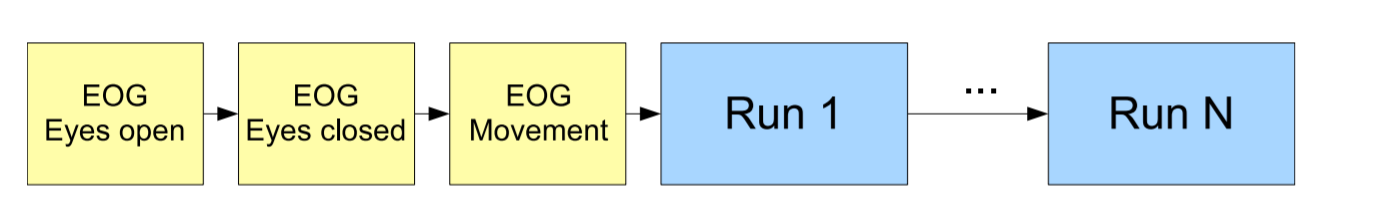
\includegraphics[scale=0.5]{./figuras/graz-eog}
 	\label{fig:Graz-EOG}
 \end{figure}
 \par 
 Os primeiros 5 minutos de cada sess\~ao foram gravados para estimar o efeito do \ac{EOG} no sinal \ac{EEG}.
 Este per\'iodo de grava\c{c}\~ao foi divido em 3 blocos: (1) dois minutos com os olhos abertos (olhando num marcador fixo) (2) um minuto com os olhos fechados e (3) um minuto com os olhos em movimento.
 Este bloco de \ac{EOG} n\~ao est\'a dispon\'ivel para as sess\~oes   B0102T e B0504E, de acordo com a fonte, devido a problemas t\'ecnicos.
 \par
  No processo de grava\c{c}\~ao foram utilizados 3 canais bipolares (C3,Cz e C4) com uma frequ\^encia de amostragem de 250Hz.
 As grava\c{c}\~oes t\'em faixa din\^amica de $\pm 100 \mu$V para as sess\~oes sem feedback e $\pm 50 \mu$V para as sess\~oes com feedback. Elas foram filtrados com um passa-faixa de 0.5Hz a 100Hz e um filtro notch em 50Hz (para reduzir o ru\'ido da rede el\'etrica). O posicionamento para cada um dos eletrodos variou ligeiramente em cada um dos sujeitos.
 Tamb\'em foi gravado o \ac{EOG} com tr\^es eletrodos monopolares usando a mesmas configura\c{c}\~oes de amplica\c{c}\~ao mas com uma faixa din\^amica maior de $\pm 1$mV.
 \par
  \begin{figure}[h!]
 	\caption{Os dois tipos de sess\~ao em Graz-b \cite{GrazBData}. }  	
  	\centering
 	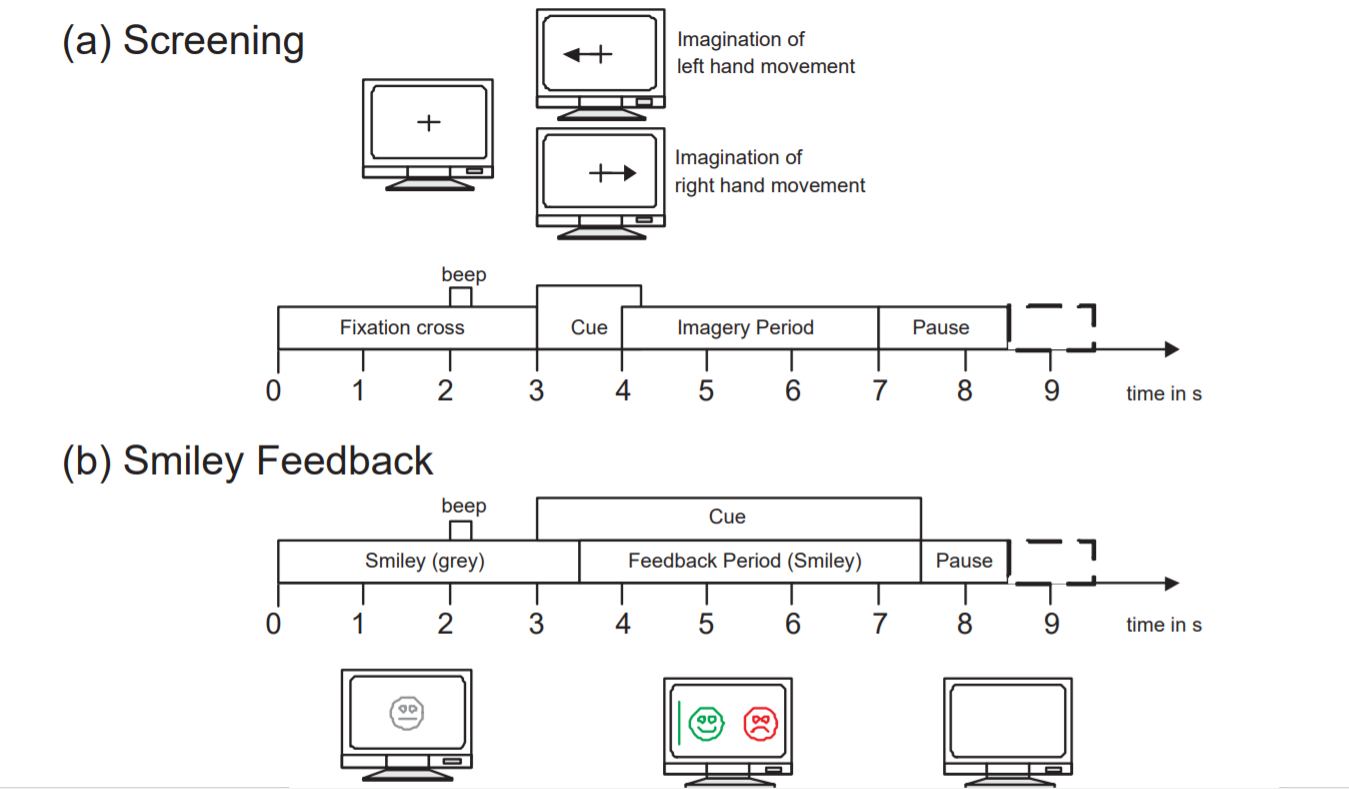
\includegraphics[scale=0.5]{./figuras/graz_b_session}
 	\label{fig:Graz-Session}
 \end{figure}
 As sess\~oes podem divididas em dois tipos
\begin{enumerate}[label=(\alph*)]
	\item \textbf{Sess\~oes sem feedback}: 
	Estas sess\~oes consistem em 6 s\'eries contendo 10 experimentos de cada uma das duas categorias, dando um total de 120 experimentos.
	Neste experimento, nos primeiros 3 segundos foi exibido uma cruz de fixa\c{c}\~ao com um curto aviso sonoro.
	Depois disso uma seta apontando para direita ou esquerda (dependendo do tipo de a\c{c}\~ao motora imagin\'aria) foi utilizado como deixa durando 1.25s .
	 Posteriormente o sujeito teve um período de 4 segundos para imaginar o movimento da m\~ao correspondente ao lado da seta.
	 Para finalizar cada experimento foi seguido por uma parada aleat\'oria de 1.5 a 2.5 segundos para evitar de que o sujeito se adapte.
	\item \textbf{Sess\~oes com feedback}:
	Estas sess\~oes consistiram em 4 s\'eries de 20 experimentos para cada tipo de imagina\c{c}\~ao motora dando um total de 160 experimentos. 
	No inicio deste tipo de sess\~ao foi centralizado um smiley cinza na tela e no segundo posterior foi acionado um aviso sonoro. Ap\'os mais um segundo a deixa foi apresentada dependendo da deixa os sujeitos foram pedidos para moverem o smiley para a direita ou esquerda dando um per\'iodo de 4.5 segundos para imaginar esta a\c{c}\~ao. Caso o smiley fosse movido para o lado correto ele ficaria verde caso contrario vermelho.
	Depois disso, um periodo alet\'orio de 1-2 segundos foi adicionado a cada experimento.
\end{enumerate}
\clearpage
\section{Framework}
\par
Para fazer a compara\c{c}\~ao entre as metodologias  de extra\c{c}\~ao de caracter\'istica e classificadores foi desenvolvido um \textit{framework} para automatizar o processo de treinamento e compara\c{c}\~ao. Este \textit{framework} foi projetado com programa\c{c}\~ao \ac{OOP} em mente devido \`a sua modularidade e f\'acil expans\~ao.
\subsection{Compare Methods}
A fun\c{c}\~ao \textit{CompareMethods} compara todas as configura\c{c}\~oes fornecidas, gera uma tabela com as configura\c{c}\~oes e retorna os classificadores treinados.
\begin{figure}[h!]
	\caption{diagrama compare methods}	
	\centering
	\tikzstyle{block} = [
		% The shape:
		rectangle split,
		rectangle split parts =1,
		% The size:
		minimum size=6mm,
		draw,
		text badly centered,
		draw=blue!80!black!40,
		text=black,
	]
\tikzstyle{decision} = [
		diamond,
		draw,
		text badly centered,
		color=blue,
		aspect=2,
		inner sep=1.5pt,
		scale=0.7,
]
\tikzstyle{begin} = [
		rounded rectangle,
		draw,
		text badly centered,
		minimum size = 1cm,
		color=blue,
]
\tikzstyle{input} = [
ellipse,
draw,
text badly centered,
minimum size = 1cm,
color=blue,
]
\tikzstyle{coord} = [
-stealth,
inner sep =0 pt,
]
\begin{tikzpicture}[node distance= 0.6cm,
transition/.style={very thick,->}
]

\node [begin] (start) {\textbf{In\'icio itera\c{c}\~ao}};
\node[block,rectangle split parts=2] (Sujeito) [below=of start] {\nodepart{one}Sele\c{c}\~ao
	 \nodepart{two} Sujeito};
\node[block,rectangle split parts=2] (DB) [below=of Sujeito]{\nodepart{one}Obten\c{c}\~ao \nodepart{two} Database};
\node[block,rectangle split parts=2] (Dataset) [below=of DB] {\nodepart{one} Obten\c{c}\~ao
\nodepart{two} Dataset};
\node[block,rectangle split parts=1](Train) [below=of Dataset]{
	\nodepart{one} Treinamento classificador
};
\node[block,rectangle split parts=1] (Avaliacao1) [below=of Train]{Avalia\c{c}\~ao performance por Janela amostrada};
%\node []
\draw [transition] (start) -> (Sujeito);
\draw [transition] (Sujeito) -> (DB);
\draw [transition] (DB) -> (Dataset);
\draw [transition] (Dataset) -> (Train);
\draw [transition] (Train) -> (Avaliacao1);
\end{tikzpicture}
	\label{fig:comparemethods}
\end{figure}
\subsection{Trials}
\begin{figure}[h!]
	\caption{diagrama do Trials}	
	\centering
	\tikzstyle{class} = [rectangle split,rectangle split parts=1,draw ,text badly centered, node distance=1cm,scale=0.9]
\begin{tikzpicture}
[edge from parent fork down,sibling distance=4cm,level distance=7cm,
edge from parent/.style={draw,<-,line width=1.2pt}]
\node[class,rectangle split parts=2](Database)
	{
	\nodepart{one}  \textcolor{blue}{\large{Trials}}
	 \nodepart{two} \begin{tabular}{cc}
					\textcolor{purple}{Trials}(path)\\
					\textcolor{purple}{Trials}(path,labels)\\
					\end{tabular}
				
};
\end{tikzpicture}
	\label{fig:Trials}
\end{figure}
%\begin{table}[h!]
%	\centering
%	\caption{M\'etodos da classe Trials}
%	\begin{tabularx}{\textwidth}{c|X}
%		
%		\hline\hline
%		METODO & DESCRI\c{C}\~AO \\ \hline 
%		\textcolor{purple}{Trials} &  \\ \hline
%	\end{tabularx}
%	\label{Tab:metodostrials}
%\end{table}
\textbf{Trials} durante a cria\c{c}\~ao pega o arquivo contendo a sess\~ao de \ac{EEG} filtra os canais de artefatos \ac{EOG} nos canais \ac{EEG} (C3,Cz,C4) usando a \textit{regress\~ao linear} de \cite{EOG2006}, posteriormente ele extrai os experimentos e associa a categoria de imagina\c{c}\~ao motora (1) esquerda e (2) direita ao experimento. Essa informac\~ao \'e obtida do arquivo da sess\~ao ou \'e fornecida atrav\'ez do argumento \textit{labels}.
%\clearpage
\subsection{Database}
\par O \textbf{Database} \'e a classe respons\'avel por fazer a amostragem, extra\c{c}\~ao de caracter\'isticas e de maneira geral preparar os dados para serem utilizados por um classificador. O processo de prepara\c{c}\~ao dos dados para treinamento e valida\c{c}\~ao \'e o seguinte (figura \ref{fig:processoamostragem})
\begin{enumerate}
	\item Durante cria\c{c}\~ao do objeto do tipo \textbf{Database}, cada experimento  armazenado em \textit{Trials} \'e dividido em v\'arias janelas de amostragem com dura\c{c}\~ao $windowLength$ e cada janela tem uma porcentagem de sobreposi\c{c}\~ao com a janela anterior determinada por $overlap$.
	\item As janelas de amostragem s\~ao armazenadas junto com as classifica\c{c}\~oes obtidas do objeto Trials.
	\item \'E gerado um vetor contendo os ind\'ices de amostras aleat\'orias contendo um n\'umero igual de amostras para cada categoria.
	\item De cada janela de amostragem s\~ao extra\'ido os vetores de caracter\'isticas usando a fun\c{c}\~ao de extra\c{c}\~ao de caracter\'isticas configurada. \'E retornado uma matriz contendo o Dataset seguindo o padr\~ao em que os vetores de caracter\'isticas est\~ao nas linhas e na \'ultima coluna consta a categoria da amostra.
\end{enumerate}
\begin{equation}
\left[
\begin{array}{cccc}
F(C3_1) &  F(Cz_1) & F(C4_1) & Cat_1\\ 
F(C3_2) &  F(Cz_2) & F(C4_2) & Cat_2\\ 
\vdots & \vdots & \vdots &\vdots \\
F(C3_n) &  F(Cz_n) & F(C4_n) & Cat_n\\ 
\end{array}
\right]
\end{equation}

\begin{figure}[h!]
	\caption{Amostragem e extra\c{c}\~ao de caracter\'itsticas}	
	\centering
	\tikzstyle{sample}=[minimum height=1cm,minimum width=4cm,xshift=2cm,draw=black]
\tikzstyle{plotsf}=[smooth,yscale=0.05,xscale=8,color=blue]
%\tikzstyle{lines}=[color=black,line width=0.5mm]
\tikzstyle{lines}=[color=black,very thick]
\begin{tikzpicture}[
 brc/.style args = {#1/#2}{decorate,
	decoration={brace, amplitude=5pt,
		raise=#1,#2},% for mirroring of brace
	thick},]
%\begin{axis}[axis line style={draw=none},
%tick style={draw=none},]
%	\addplot table[y=y,x=t,col sep=comma] {./dados/EEG2.csv};
%\end{axis}
\draw (0,0)  [plotsf] plot file {./dados/EEG2.table};
\draw [lines, dashdotted ](2cm,0.5cm)--(2cm,-4cm);
\draw [lines, dashdotted ](4cm,0.5cm)--(4cm,-4cm);
\draw [lines](2cm,-3.5cm)--(4cm,-3.5cm) node [midway,below] {\textbf{overlap}};
\draw [thick,double,->] (4.5cm,-3cm)--(4.5cm,-4cm)--(10cm,-4cm) node [midway,below]{\tiny{\textbf{Extra\c{c}\~ao de caracter\'isticas}}};
\draw (0,0) node (s0) [sample,minimum width=16cm,xshift=6cm]{};
\begin{scope}[yshift=-1.25cm]
\draw (0,0) [plotsf] plot file {./dados/EEG1-1.table};
\draw (0,0) node (s1) [sample] {};
\end{scope}
\node (s1text) [right=of s1,xshift=-1cm]{Janela 1};
\begin{scope}[yshift=-2.5cm]
\draw (0,0)[plotsf] plot  file {./dados/EEG1-2.table};
\draw (0,0) node (s2) [sample,xshift=2cm] {};
\end{scope}
\node (s1text) [right=of s2,xshift=-1cm]{Janela 2};
\begin{scope}[xshift=10cm,yshift=-5cm]
\begin{scope}[scale=0.6]
\begin{axis}[%axis line style={draw=none},
tick style={draw=none},
]
	\addplot table[y=P,x=f,col sep=comma] {./dados/EEGWelch2.csv};
\end{axis}
\end{scope}
\end{scope}
\draw[brc=2mm/](0,0.5)--(16,0.5) node [midway,above,yshift=6]{\textbf{Experimento}};
\end{tikzpicture}
	\label{fig:processoamostragem}
\end{figure}
\begin{figure}[h!]
	\caption{diagrama do Database}	
	\centering
	\tikzstyle{class} = [rectangle split,rectangle split parts=1,draw ,text badly centered, node distance=1cm,scale=0.9]
\begin{tikzpicture}
[edge from parent fork down,sibling distance=4cm,level distance=7cm,
edge from parent/.style={draw,<-,line width=1.2pt}]
\node[class,rectangle split parts=2](Database)
	{
	\nodepart{one}  \textcolor{blue}{\large{Database}}
	 \nodepart{two} \begin{tabular}{cc}
					\textcolor{purple}{Database}(overlap,windowLength,Trials)\\
					\textcolor{purple}{getSampleCountPerLabel}()\\
					\textcolor{purple}{generateDatasetIndex}(numSamples)\\
					\textcolor{purple}{generateDataset}(TrainingDataset)\\
					\textcolor{purple}{getSample}(Range)\\
					\textcolor{purple}{getSampleCount}()\\
					\textcolor{purple}{setFeatureExtractionFcn}(FEFunction)\\
					\end{tabular}
				
};
\end{tikzpicture}
	\label{fig:Database}
\end{figure}
\begin{table}[h!]
	\centering
	\caption{M\'etodos da classe Database}
	\begin{tabularx}{\textwidth}{c|X}		
		\hline\hline
		METODO & DESCRI\c{C}\~AO \\ \hline 
		\textcolor{purple}{Database} & Cria um objeto da classe Database contendo as amostras do objeto da classe Trials usando os par\^ametros \textit{overlap} e \textit{windowLength} para gerar as amostras. \\ \hline
		\textcolor{purple}{getSampleCountPerLabel} & Retorna a quantidade de janelas de amostragem de cada categoria\\ \hline
		\textcolor{purple}{generateDatasetIndex} &  Gera o \'indice do dataset contendo o n\'umero de janelas de amostragem \textit{numSamples}\\ \hline
		\textcolor{purple}{generateDataset} & Retorna o dataset contendo os vetores de caracter\'isticas seguido pelas suas categorias \\ \hline
		\textcolor{purple}{getSample} & Retorna as janelas de amostragem com o seus \'indices determinado por \textit{Range} \\ \hline
		\textcolor{purple}{getSampleCount} &  Retorna o n\'umero total de janelas de amostragem\\\hline
		\textcolor{purple}{setFeatureExtractionFcn} & Configura a func\~ao de extra\c{c}\~ao de caracter\'isticas \\ \hline
	\end{tabularx}
	\label{Tab:metodosdb}
\end{table}
\clearpage
\subsection{FeatureExtractionFnc}
\'E a classe contendo a fun\c{c}\~ao de extra\c{c}\~ao de caracter\'isticas.A fun\c{c}\~ao \textit{ExtractFeature}, virtual na classe base, foi implementada em tr\^es classes derivadas. S\~ao elas: o \acf{PWelch}, \acf{PMTM} e \ac{PSDp}. Para o \ac{PSDp} e \ac{PWelch} foram utilizadas janelas retangulares. Todas as configura\c{c}\~oes restantes s\~ao as padr\~oes do \textbf{MATLAB™}.
\begin{figure}[h!]
	\caption{diagrama de heran\c{c}a do FeatureExtractionFnc}	
	\centering
	\tikzstyle{class} = [rectangle split,rectangle split parts=1,draw ,text badly centered, node distance=1cm,scale=0.7]
\begin{tikzpicture}
[edge from parent fork down,sibling distance=5cm,level distance=4cm,
edge from parent/.style={draw,<-,line width=1.2pt}]
\node[class,rectangle split parts=2](FeatureExtractionFnc)
	{
	\nodepart{one}  \textcolor{blue}{\large{\textit{FeatureExtractionFnc}}}
	 \nodepart{two} \begin{tabular}{cc}
	 					 \textit{\textcolor{purple}{ExtractFeature}}(C3,Cz,C4)\\
					\end{tabular}
	}
	child{ node [class, rectangle split parts=2] (PWelch)
		{
		\nodepart{one} \large{\textcolor{blue}{PWelch}}
		\nodepart{two} \begin{tabular}{cc}
							\textcolor{purple}{ExtractFeature}(C3,Cz,C4)\\
						\end{tabular}
		}
	}
	child{ node [class, rectangle split parts=2] (PSD)
		{
		\nodepart{one} \large{\textcolor{blue}{PSD}}
		\nodepart{two} \begin{tabular}{cc}
		\textcolor{purple}{ExtractFeatures}(C3,Cz,C4)\\
		\end{tabular}
		}
	}
	child{ node [class, rectangle split parts=2] (PMTM)
		{
		\nodepart{one} \large{\textcolor{blue}{PMTM}}
		\nodepart{two} \begin{tabular}{cc}
		\textcolor{purple}{ExtractFeatures}(C3,Cz,C4)\\
		\end{tabular}
		}
	};
\end{tikzpicture}
	\label{fig:FeatureExtraction}
\end{figure}

\clearpage
\subsection{Classifier}
\begin{figure}[h!]
	\caption{diagrama de heran\c{c}a do Classifier}	
	\centering
	\tikzstyle{class} = [rectangle split,rectangle split parts=1,draw ,text badly centered, node distance=1cm,scale=0.7]
\begin{tikzpicture}
[edge from parent fork down,sibling distance=4cm,level distance=7cm,
edge from parent/.style={draw,<-,line width=1.2pt}]
\node[class,rectangle split parts=3](Classifier)
	{
	\nodepart{one}  \textcolor{blue}{\large{\textit{Classifier}}}
	 \nodepart{two} \begin{tabular}{cc}
	 					 \textit{\textcolor{purple}{train}}()\\
 						 \textit{\textcolor{purple}{predict}}()\\
					\end{tabular}
	 \nodepart{three} \begin{tabular}{cc}
					\textcolor{purple}{calculatePerformance}(ValidationSet)\\
					\textcolor{purple}{exportModel}()\\
					\textcolor{purple}{loadModel}(Model)\\
					\textcolor{purple}{loadTrainingData}(TrainingDataset)\\
					\end{tabular}
				
	}
	child{ node [class, rectangle split parts=2] (LinearSVM)
		{
		\nodepart{one} \large{\textcolor{blue}{LinearSVM}}
		\nodepart{two} \begin{tabular}{cc}
							\textcolor{purple}{LinearSVM}()\\
							\textcolor{purple}{train}()\\
							\textcolor{purple}{predict}()\\
						\end{tabular}
		}
	}
	child{ node [class, rectangle split parts=2] (gaussianSVM)
		{
		\nodepart{one} \large{\textcolor{blue}{gaussianSVM}}
		\nodepart{two} \begin{tabular}{cc}
		\textcolor{purple}{gaussianSVM}(KernelScale)\\
		\textcolor{purple}{train}()\\
		\textcolor{purple}{predict}()\\
		\end{tabular}
		}
	}
	child{ node [class, rectangle split parts=2] (kNN)
		{
		\nodepart{one} \large{\textcolor{blue}{kNN}}
		\nodepart{two} \begin{tabular}{cc}
		\textcolor{purple}{kNN}(numNeighbours)\\
		\textcolor{purple}{train}()\\
		\textcolor{purple}{predict}()\\
		\end{tabular}
		}
	}
	child{ node [class, rectangle split parts=2] (ANN)
		{
			\nodepart{one} \large{\textcolor{blue}{ANN}}
			\nodepart{two} \begin{tabular}{cc}
			\textcolor{purple}{ANN}(Layers)\\
			\textcolor{purple}{train}()\\
			\textcolor{purple}{predict}()\\
			\end{tabular}
		}
};
\end{tikzpicture}
	\label{fig:Classifier}
\end{figure}
\begin{table}[h!]
	\centering
	\caption{M\'etodos da classe Classifier}
	\begin{tabularx}{\textwidth}{c|X}
		
		\hline\hline
		METODO & DESCRI\c{C}\~AO \\ \hline 
		\textcolor{purple}{train} & Treina o classificador  \\ \hline
		\textcolor{purple}{predict} & Determina a classifica\c{c}\~ao dos dados de entrada \\ \hline
		\textcolor{purple}{calculatePerformance} & Aceita o par\^ametro ValidationSet, contendo o conjunto de valida\c{c}\~ao e retorna a performance do classificador em percentual de acertos e $\kappa$ de Cohen. \\ \hline
		\textcolor{purple}{exportModel} & Exporta o modelo do classificador \\ \hline
		\textcolor{purple}{loadTrainingData} & Carrega o conjunto de treinamento TrainingDataset.\\ \hline
	\end{tabularx}
	\label{Tab:metodosclass}
\end{table}
 \textbf{Classifier}  \'e uma classe abstrata que descreve os classificadores e cont\'em os m\'etodos descritos na tabela \ref{Tab:metodosclass}.
Os m\'etodos train e predict s\~ao virtuais na classe base e realizam o treinamento e a classifica\c{c}\~ao dos dados nas seguintes classes derivadas:
%Estas s\~ao \textbf{LinearSVM}, \textbf{gaussianSVM}, \textbf{kNN} e \textbf{ANN} estas classes implementam respectivamente um classificador do tipo \ac{SVM} com kernel linear, um \ac{SVM} com kernel gaussiano, \ac{kNN} e um \ac{ANN}.
\begin{enumerate}
	\item \textbf{LinearSVM} implementa um \ac{SVM} com kernel linear.
	\item \textbf{gaussianSVM} implementa um \ac{SVM} com kernel gaussiano durante a inicializa\c{c}\~ao \'e poss\'ivel especificar o par\^ametro $\gamma$ do kernel usando o argumento KernelScale
	\item \textbf{k-NN} \'e um classificador \acs{kNN} com m\'etrica euclidiana que permite, no seu construtor, a especifica\c{c}\~ao da quantidade de viz\'inhos pr\'oximos ($k$).	  
	\item \textbf{ANN} \'e uma rede neural utilizando-se da fun\c{c}\~ao de ativa\c{c}\~ao do tipo \textit{tanh}, \ac{SCG} como o m\'etodo de treinamento e a entropia cruzada como fun\c{c}\~ao de erro. O n\'umero de neur\^onios e a quantidade de camadas ocultas pode ser passada pelo argumento Layers durante a inicializa\c{c}\~ao (por padr\~ao, os objetos desta classe s\~ao configurados com duas camadas ocultas de 20 neu\^onios cada).
\end{enumerate}
\section{M\'etodos de avalia\c{c}\~ao de performance}
\par 
Foram utilizadas 2 m\'etricas de avalia\c{c}\~ao de performance.
A primeira envolve classificar janelas de amostragem isoladas e calcular o $\kappa$ de Cohen e a preci\c{c}\~ao de classifica\c{c}\~ao.
 Esta m\'etrica foi escolhida para poder analisar o impacto da redu\c{c}\~ao da largura da janela de amostragem.
\par
O segundo m\'etodo consiste em obter todas as janelas de amostragem de um experimento, classificar elas e considerar a classifica\c{c}\~ao do experimento como a moda das janelas de amostragem. Depois disso calculado o $\kappa$ de Cohen e a precis\~ao de classifica\c{c}\~ao do experimento.
 Essa m\'etrica foi usada para comparar a performance destes m\'etodos com os utilizados na competi\c{c}\~ao \ac{BCI}-IV 2008 que utilizou o mesmo dataset.